%%
% The SUEPThesis Template for Bachelor Graduation Thesis
%
% 上海电力大学毕业设计(论文)中英文摘要 —— 使用 XeLaTeX 编译
%
% Copyright 2020-2023 SUEPaper
%
% This work may be distributed and/or modified under the
% conditions of the LaTeX Project Public License, either version 1.3
% of this license or (at your option) any later version.
% The latest version of this license is in
%   http://www.latex-project.org/lppl.txt
% and version 1.3 or later is part of all distributions of LaTeX
% version 2005/12/01 or later.
%
% This work has the LPPL maintenance status `maintained'.
%
% The Current Maintainer of this work is Haiwen Zhang.
%%

\documentclass{suepthesis}

\SUEPSetup{
  cover = {
    %% 使用以下参数来自定义封面日期
    date = 2023年6月5日,
  },
  info = {
    % 想要删除某项封面信息,直接删除该项即可。
    % 想要让某项封面信息留空(但是保留下划线),请设置为空字符串。
    % 如需要换行,则用 “\\” 符号分割。
    title = 水下机器人生产和存储计划,
    % 当且仅当封面题目的第一栏写不下,再使用subtitle用于扩充
    subtitle = 问题的优化建模,
    titleEn = {Optimal modeling of production and storage planning for WPCR},
    institution = 数理学院数学系,
    class = 信息与计算科学专业2019级,
    author = 徐逸宁,
    studentId = 20192295,
    supervisor = 邓化宇,
    keywords = {动态规划;0-1规划;层次分析;遗传算法;策略迭代},
    keywordsEn = {Dynamic Programming; 0-1 Programming; Analytic Hierarchy Process; Genetic Algorithm; Strategy Iteration},
  }
}

% \usepackage[
%   backend=biber,
%   style=gb7714-2015,
%   gbalign=gb7714-2015,
%   gbnamefmt=lowercase,
%   gbpub=false,
%   doi=false,
%   url=false,
%   eprint=false,
%   isbn=false,
% ]{biblatex}

\usepackage[backend=biber,gbnamefmt=lowercase,style=gb7714-2015]{biblatex}

% 参考文献引用文件位于 content/thesis.bib
\addbibresource{content/thesis.bib}


% 文档开始
\begin{document}

% 标题页面:如无特殊需要,本部分无需改动
\MakeCover

% 原创性声明:如无特殊需要,本部分无需改动
% ====== 原创性声明(LaTeX 格式)======
\MakeOriginality
% ====== 原创性声明(LaTeX 格式)======

% 前置页面定义
\frontmatter
% 摘要:在摘要相应的 TeX 文件处进行摘要部分的撰写
%%
% The BIThesis Template for Bachelor Graduation Thesis
%
% 上海电力大学毕业设计(论文)中英文摘要 —— 使用 XeLaTeX 编译
%
% Copyright 2020-2023 SUEPaper
%
% This work may be distributed and/or modified under the
% conditions of the LaTeX Project Public License, either version 1.3
% of this license or (at your option) any later version.
% The latest version of this license is in
%   http://www.latex-project.org/lppl.txt
% and version 1.3 or later is part of all distributions of LaTeX
% version 2005/12/01 or later.
%
% This work has the LPPL maintenance status `maintained'.
%
% The Current Maintainer of this work is Haiwen Zhang.
%%

% 中英文摘要章节
\begin{abstract}
  % 中文摘要正文从这里开始
  本文……。
  
  \textcolor{blue}{摘要正文选用模板中的样式所定义的“正文”,每段落首行缩进 2 个字符;或者手动设置成每段落首行缩进 2 个汉字,字体:宋体,字号:小四,行距:1.5倍,间距:段前、段后均为 0 行。阅后删除此段。}
  
  \textcolor{blue}{摘要是一篇具有独立性和完整性的短文,应概括而扼要地反映出本论文的主要内容。包括研究目的、研究方法、研究结果和结论等,特别要突出研究结果和结论。中文摘要力求语言精炼准确,本科生毕业设计(论文)摘要建议 300-500 字。摘要中不可出现参考文献、图、表、化学结构式、非公知公用的符号和术语。英文摘要与中文摘要的内容应一致。阅后删除此段。}
  
  \end{abstract}
  
  % 英文摘要章节
  \begin{abstractEn}
  % 英文摘要正文从这里开始
  In order to study……
  
  \textcolor{blue}{Abstract 正文设置成每段落首行缩进 2 字符,字体:Times New Roman,字号:小四,行距:固定值 25 磅,间距:段前、段后均为 0 行。阅后删除此段。}
  \end{abstractEn}
  

\MakeTOC

% 正文开始
\mainmatter

%%
% The BIThesis Template for Bachelor Graduation Thesis
%
% 上海电力大学毕业设计(论文)中英文摘要 —— 使用 XeLaTeX 编译
%
% Copyright 2020-2023 SUEPaper
%
% This work may be distributed and/or modified under the
% conditions of the LaTeX Project Public License, either version 1.3
% of this license or (at your option) any later version.
% The latest version of this license is in
%   http://www.latex-project.org/lppl.txt
% and version 1.3 or later is part of all distributions of LaTeX
% version 2005/12/01 or later.
%
% This work has the LPPL maintenance status `maintained'.
%
% The Current Maintainer of this work is Haiwen Zhang.
%%

%子章节为了便于查找和修改,建议通过input拆分文件

%%%%%%%%%%%%%%%%%%%%%%%%%%%%%%%%绪论%%%%%%%%%%%%%%%%
%%
% The BIThesis Template for Bachelor Graduation Thesis
%
% 上海电力大学毕业设计(论文)中英文摘要 —— 使用 XeLaTeX 编译
%
% Copyright 2020-2023 SUEPaper
%
% This work may be distributed and/or modified under the
% conditions of the LaTeX Project Public License, either version 1.3
% of this license or (at your option) any later version.
% The latest version of this license is in
%   http://www.latex-project.org/lppl.txt
% and version 1.3 or later is part of all distributions of LaTeX
% version 2005/12/01 or later.
%
% This work has the LPPL maintenance status `maintained'.
%
% The Current Maintainer of this work is Haiwen Zhang.
%%

\chapter{一级标题}

这是上海电力大学本科学位论文\LaTeX{}模板,下面的文字主要作用为对重构后的模板样式设置进行测试。
测试样例基本覆盖模板设定,包括多级标题的基本样式,段落与缩进距离。

\section{二级标题}

\subsection{三级标题}

一级标题根据学校提供的Word模板要求,小三号黑体居中,章节号空一个汉字,段前0行,段后0.5行
并且每一章节单独起一页,章节号格式应使用中文汉字。

二级标题为黑体四号字,居左,1.5倍行距,段前0.5行,段后0行。章节号后空一个汉字。

三级标题黑体小四号字,1.5倍行距,段前0.5行,段后0行,缩进两个汉字,章节号后空一个汉字。

所有标题样式由 \textbf{suepthesis.cls} 模板文件 \textbf{ctexset} 进行设置。

\section{字体}

正文字体默认使用小四号宋体,英文为小四号 Times New Romen,各段行首缩进两个汉字



英文字体展示如下:

TeX (/tɛx, tɛk/, see below), stylized within the system as TEX, is a typesetting system (or a "formatting system") which was designed and mostly written by Donald Knuth\cite{knuth1984texbook} and released in 1978. TeX is a popular means of typesetting complex mathematical formulae; it has been noted as one of the most sophisticated digital typographical systems.


\subsection{调节字号}

可以使用 命令来调节字号。

\begin{tabular}{ll}
  \verb|\chuhao | & \chuhao  初号字 English \\
  \verb|\xiaochu| & \xiaochu 小初号 English \\
  \verb|\yihao  | & \yihao  一号字 English \\
  \verb|\xiaoyi | & \xiaoyi 小一号 English \\
  \verb|\erhao  | & \erhao  二号字 English \\
  \verb|\xiaoer | & \xiaoer 小二号 English \\
  \verb|\sanhao | & \sanhao  三号字 English \\
  \verb|\xiaosan| & \xiaosan 小三号 English \\
  \verb|\sihao  | & \sihao  四号字 English \\
  \verb|\xiaosi | & \xiaosi 小四号 English \\
  \verb|\wuhao  | & \wuhao  五号字 English \\
  \verb|\xiaowu | & \xiaowu 小五号 English \\
  \verb|\liuhao  | & \liuhao  六号字 English \\
  \verb|\xiaoliu | & \xiaoliu 小六号 English \\
  \verb|\qihao  | & \qihao  七号字 English \\
  \verb|\bahao | & \bahao 八号字 English \\

\end{tabular}

\subsection{调节字体}

需要说明的是由于Linux或者macOS系统上不包含学校写作指导要求的字体,因此我们将Windows的字体放在了fonts目录下,
由于这些字体具有版权,所以我们仍\textbf{强烈建议}您在Windows操作系统上编译最终版论文。

中文可选字体以及选用指令如下:

\begin{tabular}{l l}
  \verb|\songti| & {\songti 宋体} \\
  \verb|\heiti| & {\heiti 黑体}
\end{tabular}

我们在模板中通过调整\verb|\newCJKfontfamily|的AutoFakeBold参数来简单实现字体加粗,
在正文中你可以使用习惯的\verb|\textbf|指令来加粗对应中文。
如果你需要调整字体,也可以组合使用字体选择并加粗,比如\verb|\heiti\bfseries|

\textbf{宋体加粗测试},宋体不加粗测试。

{\heiti\bfseries 黑体加粗测试。}{\heiti 黑体不加粗测试。}

目前模板并没有按照一些其他模板写法中常见的,重定向加粗和倾斜效果到upright。


\section{模板主要结构}

本项目模板的主要结构, 如下表所示:
% TODO 进一步完善

\begin{table}[ht]
  \centering
  \begin{tabular}{r|l|l}
    \hline\hline
    \multicolumn{2}{l|}{main.tex } & 主文档,可以理解为文章入口。  \\ \hline
                                            & abstact.tex    & 中/英文摘要内容    \\ \cline{2-3}
                                            & acknowledgements.tex       & 致谢 \\ \cline{2-3}
                                            & appendix.tex       & 附录 \\ \cline{2-3}
                                            & conclusion.tex       & 结论 \\ \cline{2-3}
                                            & ref.bib       & 参考文献库 \\ \cline{2-3}
                                            & reference.tex       & 参考文献 \\ \cline{2-3}
    \raisebox{1em}{content 目录 }            & chapters 目录   & 章节内容           \\ \hline
    \multicolumn{2}{l|}{images 目录}         & 用于存放图片文件                                  \\ \hline
    \multicolumn{2}{l|}{suepthesis.cls }    & 模板入口                                          \\ \hline\hline
  \end{tabular}
\end{table}

我们不建议模板使用者更改原有模板的结构,
但如果您确实需要,请务必先充分阅读本模板的使用说明并了解相应的\LaTeX{}模板设计知识。

\newpage

人工智能在变压器故障诊断方面地应用极大地促进了诊断技术的提高。人工智能的应用可以分为专家系统和人工神经网这两个方向。

专家系统方面:

专家系统由专家知识库,推理机以及用户接口和解释机制等主要部分组成。
知识是专家系统地核心和关键,是解决问题的出发点。
专家系统利用只是实现从故障表象到故障本质的推理过程。
它具有概念明确,长于分析,推理路径清晰,易于用户参与,便于解释等显著优点。
实际上,是对人类逻辑思维模式的计算机模拟。
但专家系统也具有缺陷:

1.	知识获取困难。首先专家系统的规则表述缺乏深度,
缺乏对专家思维过程的描述。而且专家系统的学习能力低下,
人工方式获取知识的效率又很低下使得专家系统的只是难于完备,
从而制约了专家系统的发展。

2.	知识维护困难。

3.	基于知识的推理,存在“匹配冲突”和“组合爆炸”的问题。推理的速度慢,效率差,难以适应检测控制适时性的要求。

实际应用:

以关系数据库为核心构造的电气设备故障诊断专家系统,引入对象和规则知识的模糊表示处理故障及其现象存在着的模糊性,基于数据库的优化查询实现推理。用关系数据库的元素表示一个对象或一条规则,借助隶属函数及语义距离的概念进行不确定前提下的对象处理和对象匹配,能够由不完全的对象信息得出有一定隶属度要求的关于故障性质、原因的诊断结论,并有针对性的得出应相应采取的应急和跟踪措施,为设备维护提供依据。用数据关系的思想,完全由数据库管理诊断知识,从而独立于推理机理及用户,知识数据库维护简便、规则可以保持完整性和一致性、且在数据库中加入领域知识即可对系统的诊断范围进行扩充。 

由于在电力系统的故障诊断中同时存在具有随机性和模糊性的不定因素,因此单纯用概率统计或模糊数学的方法都不利于准确的映射故障的特性。现在提出一种将两者结合起来的方法,并在此基础上重新定义了诊断问题。不仅有助于解决三比值法因编码不全而难以作出结论的不足,而且比仅基于概率统计的诊断模型具有更高的正判率。这种方法利用色谱数据和电气数据进行综合诊断,得出更为具体的诊断。

近期,为了解决专家系统较难获取完备知识的瓶颈问题。提出了一种变压器故障诊断专家系统知识库的粗糙集方法。将粗糙集理论和专家系统相结合,在变压器历史故障数据所形成决策表的简约基础上,通过计算规则的粗糙隶属度,建立了具有不同简化层次上符合置信度要求的节点网络规划集的知识库。

人工神经网方面:人工神经网将已有的数据和已知的故障诊断模式作为样本,通过学习得出数据量和故障模式间的映射关系。在神经网络系统中,信息的存储和处理是合为一体的,能从不完全的,不精确的信息联想出完整的信息,因而神经网络具有很强的学习能力,信息处理能力和学习过程中的完善性能。但是,它也有以下缺陷:


%%%%%%%%%%%%%%%%%%%%%%%%%%%%%%%%绪论%%%%%%%%%%%%%%%%

% %%%%%%%%%%%%%%%%%%%%%%%%%%%%%%%%图像插入示例%%%%%%%%%%%%%%%%
%!TEX root = ../../csuthesis_main.tex
\chapter{图表示例}

\section{图片与布局}

\subsection{插图}

图片可以通过\cs{includegraphics}指令插入,我们建议模板使用者将文章所需插入的图片源问卷放置在 images 目录中,
另外,矢量图片应使用PDF格式,位图照片则应使用JPG格式(LaTeX不支持TIFF格式)。具有透明背景的栅格图可以使用PNG格式。
模板已经配置了相对路径,所以在文中插图片时,直接用 images 目录下的相对路径即可,比如 images/csu.png ,
在正文中插入只需要\cs{includegraphics{csu.png}},不需要再增加前缀。

下面是一个简单的插图示例。

\begin{figure}[hbt]
    \centering
    
\includegraphics[width=0.3\linewidth]{logo.png}
    \caption{插图示例}
    \label{f.example}
\end{figure}


如果一个图由多个分图(子图)组成,应通过(a),(b),(c)进行标识并附注在分图(子图下方)。

\subsection{横向布局}

模板提供常见的图片布局,比如单图布局\ref{f.example},另外还有横排布局如下:

\begin{figure}[!htb]
    \centering
    \begin{subfigure}[t]{0.24\linewidth}
        \captionsetup{justification=centering}
        \begin{minipage}[b]{1\linewidth}
        
\includegraphics[width=1\linewidth]{logo.png}
        \caption{test}
        \end{minipage}
    \end{subfigure}
    \begin{subfigure}[t]{0.24\linewidth}
        \captionsetup{justification=centering}
        \begin{minipage}[b]{1\linewidth}
        
\includegraphics[width=1\linewidth]{logo_black.png}
        \caption{test}
        \end{minipage}
    \end{subfigure}
    \begin{subfigure}[t]{0.24\linewidth}
        \captionsetup{justification=centering}
        \begin{minipage}[b]{1\linewidth}
        
\includegraphics[width=1\linewidth]{logo.png}
        \caption{test}
        \end{minipage}
    \end{subfigure}
    \begin{subfigure}[t]{0.24\linewidth}
        \captionsetup{justification=centering}
        \begin{minipage}[b]{1\linewidth}
        
\includegraphics[width=1\linewidth]{logo_black.png}
        \caption{test}
        \end{minipage}
    \end{subfigure}
    \caption{图片横排布局示例}
    \label{f.row}
\end{figure}

\subsection{纵向布局}

纵向布局如图\ref{f.col}

\begin{figure}[!htb]
    \centering
    \begin{subfigure}[t]{0.15\linewidth}
        \captionsetup{justification=centering} %ugly hacks
        \begin{minipage}[b]{1\linewidth}
        
\includegraphics[width=1\linewidth]{logo.png}
        \caption{test}
        \end{minipage}
    \end{subfigure}\\
    \begin{subfigure}[t]{0.15\linewidth}
        \captionsetup{justification=centering} %ugly hacks
        \begin{minipage}[b]{1\linewidth}
        
\includegraphics[width=1\linewidth]{logo_black.png}
        \caption{test}
        \end{minipage}
    \end{subfigure}
    \caption{图片纵向布局示例}
    \label{f.col}
\end{figure}

\subsection{竖排多图横排布局}

\begin{figure}[!htb]
    \centering
    \begin{subfigure}[t]{0.13\linewidth}
        \captionsetup{justification=centering} 
        \begin{minipage}[b]{1\linewidth}
        
\includegraphics[width=1\linewidth]{logo.png} 
        \vspace{-1ex} \vfill
        
\includegraphics[width=1\linewidth]{logo_black.png}
        \caption{aaa}
        \end{minipage}
    \end{subfigure}
    \begin{subfigure}[t]{0.13\linewidth}
        \captionsetup{justification=centering} 
        \begin{minipage}[b]{1\linewidth}
        
\includegraphics[width=1\linewidth]{logo_black.png} 
        \vspace{-1ex} \vfill
        
\includegraphics[width=1\linewidth]{logo.png}
        \caption{bbb}
        \end{minipage}
    \end{subfigure}
    \caption{图片竖排多图横排布局}
    \label{f.csu_col_row}
\end{figure}

竖排多图横排布局如图\ref{f.csu_col_row}所示。注意看(a)、(b)编号与图关系


\subsection{横排多图竖排布局}

中南大学由原湖南医科大学、长沙铁道学院与中南工业大学于2000年4月合并组建而成。原中南工业大学的前身为创建于1952年的中南矿冶学院,原长沙铁道学院的前身为创建于1953年的中南土木建筑学院,两校的主体学科最早溯源于1903年创办的湖南高等实业学堂的矿科和路科。原湖南医科大学的前身为1914年创建的湘雅医学专门学校,是我国创办最早的西医高等学校之一。中南大学秉承百年办学积淀,顺应中国高等教育体制改革大势,弘扬以“知行合一、经世致用”为核心的大学精神,力行“向善、求真、唯美、有容”的校风,坚持自身办学特色,服务国家和社会重大需求,团结奋进,改革创新,追求卓越,综合实力和整体水平大幅提升。

\begin{figure}[!htb]
    \centering
    \begin{subfigure}[t]{0.3\linewidth}
        \captionsetup{justification=centering} 
        \begin{minipage}[b]{1\linewidth}
        
\includegraphics[width=0.45\linewidth]{logo.png}
        
\includegraphics[width=0.45\linewidth]{logo_black.png}
        \caption{}
        \end{minipage}
    \end{subfigure}\\
    \begin{subfigure}[t]{0.3\linewidth}
        \captionsetup{justification=centering} 
        \begin{minipage}[b]{1\linewidth}
        
\includegraphics[width=0.45\linewidth]{logo_black.png}
        
\includegraphics[width=0.45\linewidth]{logo.png}
        \caption{}
        \end{minipage}
    \end{subfigure}
    \caption{图片横排多图竖排布局}
    \label{f.csu_row_col}
\end{figure}

横排多图竖排布局如图\ref{f.csu_row_col}所示。注意看(a)、(b)编号与图关系。

\subsection{2x2图片布局}

\begin{figure}[!htb]
    \centering
    \begin{subfigure}[t]{0.3\linewidth}
        \captionsetup{justification=centering}
        \begin{minipage}[b]{1\linewidth}
            \centering
            
\includegraphics[width=0.45\linewidth]{logo.png}
            \caption{}
        \end{minipage}
    \end{subfigure}
    \hspace{-5em}
    \begin{subfigure}[t]{0.3\linewidth}
        \captionsetup{justification=centering}
        \begin{minipage}[b]{1\linewidth}
            \centering
            
\includegraphics[width=0.45\linewidth]{logo_black.png}
            \caption{}
        \end{minipage}
    \end{subfigure}\\
    \begin{subfigure}[t]{0.3\linewidth}
        \captionsetup{justification=centering}
        \begin{minipage}[b]{1\linewidth}
            \centering
            
\includegraphics[width=0.45\linewidth]{logo.png}
            \caption{}
        \end{minipage}
    \end{subfigure}
    \hspace{-5em}
    \begin{subfigure}[t]{0.3\linewidth}
        \captionsetup{justification=centering}
        \begin{minipage}[b]{1\linewidth}
            \centering
            
\includegraphics[width=0.45\linewidth]{logo_black.png}
            \caption{}
        \end{minipage}
    \end{subfigure}
    \caption{图片2x2布局}
    \label{f.csu_2x2}
\end{figure}

\newpage

\section{图表编号}

本节主要阐述在图表下侧的编号,以及引用时的编号设置问题。
使用在上一节(上一个section, \verb|\section{插图}| )中引入的图\ref{f.example},
以及在本节加入下方新图片对比来说明。

\begin{figure}[hbt]
    \centering
    
\includegraphics[width=0.3\linewidth]{logo.png}
    \caption{图标编号示例}
    \label{f.example.2}
\end{figure}

可以看到在上一节“插图示例”的编号为图\ref{f.example}。
而在本节“图标编号示例”为图\ref{f.example.2}。

% %%%%%%%%%%%%%%%%%%%%%%%%%%%%%%%%图像插入示例%%%%%%%%%%%%%%%%


%%%%%%%%%%%%%%%%%%%%%%%%%%%%%%%%表格插入示例%%%%%%%%%%%%%%%%
%%
% The SUEPThesis Template for Bachelor Graduation Thesis
%
% 上海电力大学毕业设计(论文)中英文摘要 —— 使用 XeLaTeX 编译
%
% Copyright 2020-2023 SUEPaper
%
% This work may be distributed and/or modified under the
% conditions of the LaTeX Project Public License, either version 1.3
% of this license or (at your option) any later version.
% The latest version of this license is in
%   http://www.latex-project.org/lppl.txt
% and version 1.3 or later is part of all distributions of LaTeX
% version 2005/12/01 or later.
%
% This work has the LPPL maintenance status `maintained'.
%
% The Current Maintainer of this work is Haiwen Zhang.
%%

\chapter{连续多周生产统筹规划的WPCR生产和存储模型}

\section{连续多周生产统筹规划模型的建立}

令$V_{i-1}$为状态变量,表示第$i$天开始时的库存量;$x_i$为决策变量,表示第$i$天的生产量。
状态转移方程为
\begin{equation*}
    v_i=v_{i-1}+x_i-d_i \qquad i=1,2,...,n
\end{equation*}

最优值函数$f_i(v_i)$表示从第一天初始库存量为$0$到第$i$天末库存量为$v_i$时的最小总费用,
因而可写出顺序递推关系式\cite{韩中庚2007实用运筹学模型}:
\begin{equation}
    f_i(v_i)=\mathop{\min}_{0\leq x_i \leq \sigma_i}[C_i(x_i)+h_i(v_i)+f_{i-1}(V_{i-1})] \qquad i=1,2,...,n
\end{equation}

其中,
\begin{equation}
    \sigma_i=\min(v_i+d_i,m)
\end{equation}

不允许缺货的WPCR生产和存储模型在无存货无结余的情况下进行一周(7天)的机器人的组装计划,
求解总成本最小。

然而,事实上,组件A、B、C需要提前一天生产入库才能组装WPCR,
A1、A2、A3、B1、B2、C1、C2、C3也需要提前一天生产入库才能组装A、B、C。
在连续多周生产情况下,需要统筹规划。
由不允许缺货的WPCR生产和存储模型的求解结果列出库存量和生产准备成本如下:
\begin{equation}
    v_k=v_{k-1}+x_k-d_k
\end{equation}
\begin{equation}
    C_k(x_k)=\begin{cases}
        0, & x_k=0 \\
        K+c_j \cdot x_k, & x_k=1,2,...,n \\
        \infty, & x_k > m
    \end{cases}
\end{equation}

$d_k$表示第$k$阶段对组件的需求量,$v_k$表示第$k$阶段结束时组件库存量,$m$表示每个阶段最多能生产该组件的上限数。
\begin{equation}
    \min g = \sum_{n}^{k=1}[C_k(x_k)+h_k(v_k)]
\end{equation}
\begin{equation}
    \begin{cases}
        v_0=0,v_n=0 \\
        v_k=\sum_{k}^{i}(x_i - d_i) \ge 0 & k=2,3,...,n-1 \\
        0 \leq x_k \leq m & k=1,2,...,n \\
        x_k \text{为整数} & k=1,2,...,n
    \end{cases}
\end{equation}

$h_k(v_k)$表示第$k$阶段结束时有库存量$v_k$所需的存储费用。
\begin{equation}
    y_k=\begin{cases}
        1, & x_k > 0, \text{表示生产}x_k,\text{生产准备费不为}0 \\
        0, & x_k = 0, \text{表示不生产}x_k,\text{生产准备用费为}0 
    \end{cases}
\end{equation}
\begin{equation}
    C=\sum_{n}^{k=1}[C_k(x_k)+h_k{v_k}]=\sum_{k=1}^{n}[K \cdot y_k + c_j \cdot x_k]
\end{equation}

对于WPCR而言,
\begin{equation}
    v_k=v_{k-1} + x_k - d_k    
\end{equation}

对于A,B,C组件而言,根据A,B,C生产与组装关系,有
\begin{equation}
    v_{k+2}^A=v_{k+1}^A + x_{k+2}^A - 3x_{k+2}
\end{equation}
\begin{equation}
    v_{k+2}^B=v_{k+1}^B + x_{k+2}^B - 4x_{k+2}
\end{equation}
\begin{equation}
    v_{k+2}^C=v_{k+1}^C + x_{k+2}^C - 5x_{k+2}
\end{equation}

同理,对于A1、A2、A3、B1、B2、C 1、C2、C3可以类似研究,设生产一件WPCR所需要的
A1、A2、A3、B1、B2、C1、C2、C3分别为$u_{A1}$,$u_{A2}$,$u_{A3}$,$u_{B1}$,
$u_{B2}$,$u_{C1}$,$u_{C2}$,$u_{C3}$,则
\begin{equation}
    v_{k+1}^{Ai}=v_k^{Ai} + x_{k+1}^{Ai} - u_{Ai}3x_k,\quad i=1,2,3
\end{equation}
\begin{equation}
    v_{k+1}^{Bi}=v_k^{Bi} + x_{k+1}^{Bi} - u_{Bi}3x_k,\quad i=1,2
\end{equation}
\begin{equation}
    v_{k+1}^{Ci}=v_k^{Ci} + x_{k+1}^{Ci} - u_{Ci}3x_k,\quad i=1,2,3
\end{equation}

$s.t.$
\begin{equation}
    3x_{k+2}^A+5x_{k+2}^B+5x_{k+2}^C \leq T_k
\end{equation}
\begin{equation}
    y_k=\begin{cases}
        1, & x_k > 0, \text{表示生产}x_k,\text{生产准备费不为}0 \\
        0, & x_k = 0, \text{表示不生产}x_k,\text{生产准备用费为}0 
    \end{cases}
\end{equation}
\begin{equation}
    x_k \leq My_k
\end{equation}

则各费用为,
\begin{equation}
    C_{\uppercase\expandafter{\romannumeral1}}^{'}=
        \sum_{n}^{k=1}[C_k(x_k)+h_k{v_k}]=
        \sum_{n}^{k=1}(240y_k+5v_k)
\end{equation}
\begin{equation}
    C_{\uppercase\expandafter{\romannumeral2}}^{'}=
        \sum_{n}^{k=1}(120y_{k+2}^A+2v_{k+2}^A+160y_{k+2}^B+1.5v_{k+2}^B+180y_{k+2}^C+1.7v_{k+2}^C)
\end{equation}

\begin{equation}
    \begin{aligned}
        C_{\uppercase\expandafter{\romannumeral3}}^{'} &= 
            \sum_{k=1}^{n}(40y_{k+1}^{A1}+5v_{k+1}^{A1}+60y_{k+1}^{A2}+3v_{k+1}^{A2}+50y_{k+1}^{A3}+6v_{k+1}^{A3}) \\
            &+ \sum_{k=1}^{n}(80y_{k+1}^{B1}+4v_{k+1}^{B1}+100y_{k+1}^{B2}+5v_{k+1}^{B2}) \\
            &+ \sum_{k=1}^{n}(60y_{k+1}^{C1}+3v_{k+1}^{C1}+40y_{k+1}^{C2}+2v_{k+1}^{C2}+70y_{k+1}^{C3}+3v_{k+1}^{C3})
    \end{aligned}
\end{equation}



汇总三式得目标函数为
\begin{equation}
    \min\sum_{k=1}^{n}(
            C_{\uppercase\expandafter{\romannumeral1}}^{'}+
            C_{\uppercase\expandafter{\romannumeral2}}^{'}+
            C_{\uppercase\expandafter{\romannumeral3}}^{'}) 
\end{equation}

\section{连续多周生产统筹规划模型的求解}

基于以下表\ref{T.ch3-1}的连续30周的WPCR需求的数据,
带入到连续多周生产统筹规划模型中并求解,得出表\ref{T.ch3-2}的求解结果表格。

\begin{longtable}[c]{c*{7}{r}}
    \caption{考虑检修的生产和存储模型求解结果展示}
    \label{T.ch3-1} \\
    \toprule
    \textbf{天} & \textbf{周一} & \textbf{周二} & \textbf{周三} & 
    \textbf{周四} & \textbf{周五} & \textbf{周六} & \textbf{周日} \\
    \midrule
    \endfirsthead
    \multicolumn{8}{l}{\textbf{续表~\thetable}} \\

    \toprule
    \textbf{天} & \textbf{周一} & \textbf{周二} & \textbf{周三} & 
    \textbf{周四} & \textbf{周五} & \textbf{周六} & \textbf{周日} \\
    \midrule
    \endhead
    \hline
    \multicolumn{8}{r}{续下页}
    \endfoot
    \endlastfoot
    \textbf{第1周}  & 1 & 2 & 3 & 4 & 5 & 6 & 7 \\ 
    \textbf{第2周}  & 1 & 2 & 3 & 4 & 5 & 6 & 7 \\ 
    \textbf{第3周}  & 1 & 2 & 3 & 4 & 5 & 6 & 7 \\ 
    \textbf{第4周}  & 1 & 2 & 3 & 4 & 5 & 6 & 7 \\
    \textbf{第5周}  & 1 & 2 & 3 & 4 & 5 & 6 & 7 \\
    \textbf{第6周}  & 1 & 2 & 3 & 4 & 5 & 6 & 7 \\
    \textbf{第7周}  & 1 & 2 & 3 & 4 & 5 & 6 & 7 \\
    \textbf{第8周}  & 1 & 2 & 3 & 4 & 5 & 6 & 7 \\ 
    \textbf{第9周}  & 1 & 2 & 3 & 4 & 5 & 6 & 7 \\ 
    \textbf{第10周}  & 1 & 2 & 3 & 4 & 5 & 6 & 7 \\
    \textbf{第11周}  & 1 & 2 & 3 & 4 & 5 & 6 & 7 \\
    \textbf{第12周}  & 1 & 2 & 3 & 4 & 5 & 6 & 7 \\
    \textbf{第13周}  & 1 & 2 & 3 & 4 & 5 & 6 & 7 \\
    \textbf{第14周}  & 1 & 2 & 3 & 4 & 5 & 6 & 7 \\
    \textbf{第15周}  & 1 & 2 & 3 & 4 & 5 & 6 & 7 \\
    \textbf{第16周}  & 1 & 2 & 3 & 4 & 5 & 6 & 7 \\
    \textbf{第17周}  & 1 & 2 & 3 & 4 & 5 & 6 & 7 \\
    \textbf{第18周}  & 1 & 2 & 3 & 4 & 5 & 6 & 7 \\
    \textbf{第19周}  & 1 & 2 & 3 & 4 & 5 & 6 & 7 \\
    \textbf{第20周}  & 1 & 2 & 3 & 4 & 5 & 6 & 7 \\
    \textbf{第21周}  & 1 & 2 & 3 & 4 & 5 & 6 & 7 \\
    \textbf{第22周}  & 1 & 2 & 3 & 4 & 5 & 6 & 7 \\
    \textbf{第23周}  & 1 & 2 & 3 & 4 & 5 & 6 & 7 \\
    \textbf{第24周}  & 1 & 2 & 3 & 4 & 5 & 6 & 7 \\
    \textbf{第25周}  & 1 & 2 & 3 & 4 & 5 & 6 & 7 \\
    \textbf{第26周}  & 1 & 2 & 3 & 4 & 5 & 6 & 7 \\
    \textbf{第27周}  & 1 & 2 & 3 & 4 & 5 & 6 & 7 \\
    \textbf{第28周}  & 1 & 2 & 3 & 4 & 5 & 6 & 7 \\
    \textbf{第29周}  & 1 & 2 & 3 & 4 & 5 & 6 & 7 \\ 
    \textbf{第30周}  & 1 & 2 & 3 & 4 & 5 & 6 & 7 \\ 
    \bottomrule
\end{longtable}

\begin{table}[!hpt]
    \caption{连续多周生产统筹规划的WPCR生产和存储模型求解的结果}
    \label{T.ch3-2}
    \centering
    \renewcommand\arraystretch{1.5} 
    \begin{tabular}{@{}ccccccc@{}} 
    \toprule
    \textbf{日期} & \multicolumn{1}{c}{\textbf{WPCR}} & \multicolumn{1}{c}{\textbf{A组装}} 
    & \multicolumn{1}{c}{\textbf{B组装}} & \multicolumn{1}{c}{\textbf{C组装}}
    & \multicolumn{1}{c}{\textbf{生产准备}} & \multicolumn{1}{c}{\textbf{库存}} \\
                & \multicolumn{1}{c}{\textbf{组装数量}} & \multicolumn{1}{c}{\textbf{数量}} 
    & \multicolumn{1}{c}{\textbf{数量}} & \multicolumn{1}{c}{\textbf{数量}}
    & \multicolumn{1}{c}{\textbf{费用}} & \multicolumn{1}{c}{\textbf{费用}} \\
    \midrule
    \textbf{周一} & 237 & 316 & 395 & 41 & 700 & 1619.5 \\
    \textbf{周二} & 237 & 316 & 395 & 41 & 700 & 1619.5 \\
    \textbf{周三} & 237 & 316 & 395 & 41 & 700 & 1619.5 \\
    \textbf{周四} & 237 & 316 & 395 & 41 & 700 & 1619.5 \\
    \textbf{周五} & 237 & 316 & 395 & 41 & 700 & 1619.5 \\
    \textbf{周六} & 237 & 316 & 395 & 41 & 700 & 1619.5 \\
    \textbf{周日} & 237 & 316 & 395 & 41 & 700 & 1619.5 \\
    \textbf{总和} & 237 & 316 & 395 & 41 & 700 & 1619.5 \\ 
    \bottomrule
    \end{tabular}
\end{table}



从表\ref{T.ch3-2}可以看出,连续多周生产统筹规划模型中周一、周二、周五、周六、周日的生产计划很全面,
和不允许缺货的WPCR生产和存储模型一样,如果生产计划很全面,WPCR、A、B、C都需要组装,
无论其中需要组装的数量是多少,生产准备费用都不变,都为1200元。周三只进行WPCR组装的生产计划,
而周四进行组件A、B、C的组装生产计划。总的生产和存储成本为207658元,
连续多周生产统筹规划模型平均单周所用的成本为6921.93元,
要高于不允许缺货的WPCR生产和存储模型每周的生产成本。
%%%%%%%%%%%%%%%%%%%%%%%%%%%%%%%%表格插入示例%%%%%%%%%%%%%%%%


%%%%%%%%%%%%%%%%%%%%%%%%%%%%%%%%数学公式插入示例%%%%%%%%%%%%%%%%
%!TEX root = ../../csuthesis_main.tex
\chapter{公式与符号}

中南大学由原湖南医科大学、长沙铁道学院与中南工业大学于2000年4月合并组建而成。原中南工业大学的前身为创建于1952年的中南矿冶学院,原长沙铁道学院的前身为创建于1953年的中南土木建筑学院,两校的主体学科最早溯源于1903年创办的湖南高等实业学堂的矿科和路科。原湖南医科大学的前身为1914年创建的湘雅医学专门学校,是我国创办最早的西医高等学校之一。中南大学秉承百年办学积淀,顺应中国高等教育体制改革大势,弘扬以“知行合一、经世致用”为核心的大学精神,力行“向善、求真、唯美、有容”的校风,坚持自身办学特色,服务国家和社会重大需求,团结奋进,改革创新,追求卓越,综合实力和整体水平大幅提升。

\LaTeX 的公式环境中符号样式符合 \TeX 默认的美国数学学会(AMS)的符号使用习惯,中文论文写作推荐遵循 GB/T 3102.11——1993《物理科学和技术中的数学符号》标准。这里我们给出一些 \LaTeX 中常用的符号表示。


\section{\LaTeX 数学公式模式}

\LaTeX 提供了两种数学公示的写作模式:内联模式和独显模式:

\begin{itemize}
    \item \textbf{内联模式}(inline mode),又称为行内模式,随文模式,将公式显示为段落的一部分。
    \item \textbf{独显模式}(display mode),又称为行间模式,将公式用独立行展示出来,不再作为段落的一部分。
\end{itemize}

\subsection{内联模式}

% TODO

键入如下定义符之一在段落中来使用内联模式书写数学公式符号:

\begin{itemize}
    \item \verb|\(...\)|
    \item \verb|$...$|
    \item \verb|\begin{math}...\end{math}|
\end{itemize}

\subsection{独显模式}

使用如下方式以独显模式表示数学公式:

\begin{itemize}
    \item \verb|\[...\]|
    \item \verb|\begin{displaymath}...\end{displaymath}|
    \item \verb|\begin{equation}...\end{equation}|
\end{itemize}

\textbf{公式插入示例如公式(\ref{E.example})所示。}

\begin{equation}
\gamma_{x}=
\left\{
  \begin{array}{lr}
  0, & {\rm if}~~\;|x| \leq \delta \\
  x, & {\rm otherwise}
  \end{array}
\right.
\label{E.example}
\end{equation}


\newpage


%%%%%%%%%%%%%%%%%%%%%%%%%%%%%%%%数学公式插入示例%%%%%%%%%%%%%%%%

% %%%%%%%%%%%%%%%%%%%%%%%%%%%%%%%%代码插入示例%%%%%%%%%%%%%%%%
%%
% The SUEPThesis Template for Bachelor Graduation Thesis
%
% 上海电力大学毕业设计(论文)中英文摘要 —— 使用 XeLaTeX 编译
%
% Copyright 2020-2023 SUEPaper
%
% This work may be distributed and/or modified under the
% conditions of the LaTeX Project Public License, either version 1.3
% of this license or (at your option) any later version.
% The latest version of this license is in
%   http://www.latex-project.org/lppl.txt
% and version 1.3 or later is part of all distributions of LaTeX
% version 2005/12/01 or later.
%
% This work has the LPPL maintenance status `maintained'.
%
% The Current Maintainer of this work is Haiwen Zhang.
%%

\chapter{未来订单未知情形的WPCR不确定生产和存储模型}

\section{WPCR不确定生产和存储模型的建立}

在该模型中,要求既能够保障每天的WPCR订单均以95\%以上的概率保证正常交付,
又能够以85\%以上的概率保证整周的WPCR订单能正常交付。

设划置信区间,置信区间是95\%,只要假设得到的偏差值大于0.05就说明拒绝原假设,且一周生产计划中保证85\%以上的日交付率,
如一周内至少有一天未正常交付则拒绝原假设。

设$d$为决策变量的函数,正偏差变量$d^+$表示决策值超过目标值的部分,负偏差变量$d^-$表示决策值未达到目标值的部分,
这里$d0$表示$d$的目标值。
\begin{equation}
    d^+=\max\{d-d_0,0\}
\end{equation}
\begin{equation}
    d^-=-\min\{d-d_0,0\}
\end{equation}

因决策值不可能既超过目标值同时又未达到目标值,即恒有
\begin{equation}
    d^+ \times d^- = 0
\end{equation}

设$x_k(k=1,2,...,n)$是目标规划的决策变量。设有$q$个优先级别,分别为$P_1,P_2,...,P_q$。
在同一个优先级$P$中,有不同的权重,分别记为$w_{kj}^+, w_{kj}^-(j=1,2,...,l)$。
因此目标规划模型的一般数学表达式为
\begin{equation}
    \min z=\sum_{k=1}^{q}P_k(\sum_{l}^{j=1}w_{kj}^-d_{j}^- + w_{kj}^+d_{j}^+)
\end{equation}
\begin{equation}
    \begin{cases}
        \min\sum_{k=1}^{n}(
            C_{\uppercase\expandafter{\romannumeral1}}^{'''}+
            C_{\uppercase\expandafter{\romannumeral2}}^{'''}+
            C_{\uppercase\expandafter{\romannumeral3}}^{'''}) \\
        x_k \geqslant 0 \\
        d_i^-,d_i^+\geqslant 0,i=1,2,...,l
    \end{cases}
\end{equation}

\section{WPCR不确定生产和存储模型的求解}

\subsection{WPCR不确定生产和存储模型的求解算法}

已经有研究表明策略迭代算法可以在适当的假设下产生最优(最小)成本、最优稳态控制策略和平均成本最优方程的解,且有比较好的效果。
因此本模型采用策略迭代算法进行求解。

下面给出策略迭代算法的具体实现步骤。

步骤一:初始化,$i=0$,选择初始容许控制策略。

步骤二:策略评估,$i=i+1$,控制策略$u^{i-1}$下的值函数$V^i$可以根据以下公式获得
\begin{equation}
    L(x,u^{i-1}) + (\nabla V)^{iT}(f(x)+g(x)u^{i-1})=0
\end{equation}

步骤三:策略提升,更新后的控制策略$u^i$如下
\begin{equation}
    u^i=-w(u)g^T(x)\nabla V^i
\end{equation}

步骤四:判断,若策略不满足收敛条件,那么返回步骤二继续执行,否则进入步骤五。

步骤五:结束,获得最优控制策略$u^*=u^i$和最优值函数$V^*=V^i$。
汇总上述五步,得如下策略迭代算法模拟流程图\ref{f.ch5-1}\cite{叶帅2021基于事件触发自适应动态规划的多四旋翼无人机优化控制}。

\begin{figure}[h]
    \centering
    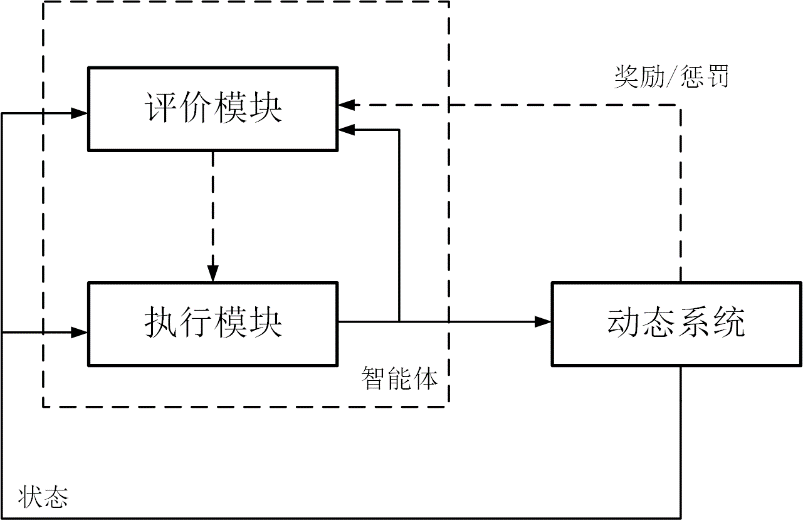
\includegraphics[width=0.5\linewidth]{ch5-1.png}
    \caption{迭代费用对比}
    \label{f.ch5-1}
\end{figure}

\subsection{WPCR不确定生产和存储模型的求解结果}

\begin{table}[H]
    \caption{WPCR不确定生产和存储模型求解的结果}
    \label{T.ch5-1}
    \centering
    \renewcommand\arraystretch{1.5} 
    \begin{tabular}{@{}ccccccc@{}} 
    \toprule
    \textbf{日期} & \multicolumn{1}{c}{\textbf{WPCR外部}} & \multicolumn{1}{c}{\textbf{A组装}} 
    & \multicolumn{1}{c}{\textbf{B组装}} & \multicolumn{1}{c}{\textbf{C组装}}
    & \multicolumn{1}{c}{\textbf{生产准备}} & \multicolumn{1}{c}{\textbf{库存}} \\
                & \multicolumn{1}{c}{\textbf{需求数量}} & \multicolumn{1}{c}{\textbf{数量}} 
    & \multicolumn{1}{c}{\textbf{数量}} & \multicolumn{1}{c}{\textbf{数量}}
    & \multicolumn{1}{c}{\textbf{费用}} & \multicolumn{1}{c}{\textbf{费用}} \\
    \midrule
    \textbf{周一} & 237 & 316 & 395 & 41 & 700 & 1619.5 \\
    \textbf{周二} & 237 & 316 & 395 & 41 & 700 & 1619.5 \\
    \textbf{周三} & 237 & 316 & 395 & 41 & 700 & 1619.5 \\
    \textbf{周四} & 237 & 316 & 395 & 41 & 700 & 1619.5 \\
    \textbf{周五} & 237 & 316 & 395 & 41 & 700 & 1619.5 \\
    \textbf{周六} & 237 & 316 & 395 & 41 & 700 & 1619.5 \\
    \textbf{周日} & 237 & 316 & 395 & 41 & 700 & 1619.5 \\
    \textbf{总和} & 237 & 316 & 395 & 41 & 700 & 1619.5 \\ 
    \bottomrule
    \end{tabular}
\end{table}

从表\ref{T.ch5-1}可以看出,该模型下,一周里面每天都有生产计划,不至于出现前几种模型中出现无生产计划的情况。
%%%%%%%%%%%%%%%%%%%%%%%%%%%%%%%%代码插入示例%%%%%%%%%%%%%%%%


% %%%%%%%%%%%%%%%%%%%%%%%%%%%%%%%%参考文献插入示例%%%%%%%%%%%%%%%%
%%
% The SUEPThesis Template for Bachelor Graduation Thesis
%
% 上海电力大学毕业设计(论文)中英文摘要 —— 使用 XeLaTeX 编译
%
% Copyright 2020-2023 SUEPaper
%
% This work may be distributed and/or modified under the
% conditions of the LaTeX Project Public License, either version 1.3
% of this license or (at your option) any later version.
% The latest version of this license is in
%   http://www.latex-project.org/lppl.txt
% and version 1.3 or later is part of all distributions of LaTeX
% version 2005/12/01 or later.
%
% This work has the LPPL maintenance status `maintained'.
%
% The Current Maintainer of this work is Haiwen Zhang.
%%

\chapter{不同情形WPCR生产和存储模型的综合分析}

\section{不同情形的WPCR生产和存储总成本比较}

通过前面四个模型优化结果可知,连续多周生产统筹规划模型相较于不允许缺货的WPCR生产和存储模型增加组装迟滞,
由图表可以看出其费用大大升高,对研究组装分配计划具有重要现实意义。
考虑检修的生产和存储模型和WPCR不确定生产和存储模型在连续多周生产统筹规划模型的基础上展开,
分别得出增设检修日期和需求未知条件下的最小费用,经对比分析,可对复杂生产中组装计划的调度具有指导意义。

\begin{figure}[h]
    \centering
    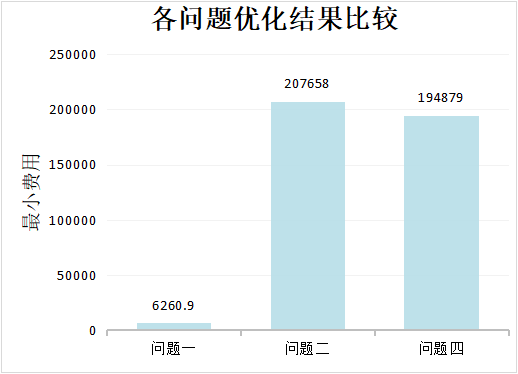
\includegraphics[width=0.7\linewidth]{ch6-1.png}
    \caption{各问题优化结果比较}
    \label{f.ch6-1}
\end{figure}

\section{不同情形的WPCR生产和存储求解的灵敏度分析}

经过灵敏度分析验证,通过遗传算法的迭代次数,以及种群数、变异率、交叉率以求得最短运行时间下的最优结果,
得出模型运算灵敏度分析,模型在大于150次迭代运算的情况下运行结果基本一致,在策略迭代中采取大种群,
在费用估计中可用最优变异交叉率来节省运算时间来求得全局最优解和动态稳定解。

\begin{figure}[H]
    \centering
    \begin{subfigure}[t]{0.5\linewidth}
        \captionsetup{justification=centering}
        \begin{minipage}[b]{1\linewidth}
            \centering
            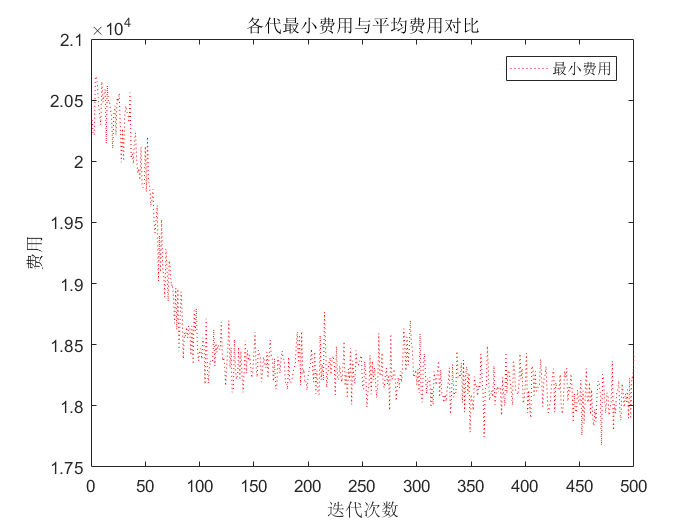
\includegraphics[width=0.8\linewidth]{ch6-2-1.png}
            \caption{}
        \end{minipage}
    \end{subfigure}
    \hspace{-5em}
    \begin{subfigure}[t]{0.5\linewidth}
        \captionsetup{justification=centering}
        \begin{minipage}[b]{1\linewidth}
            \centering
            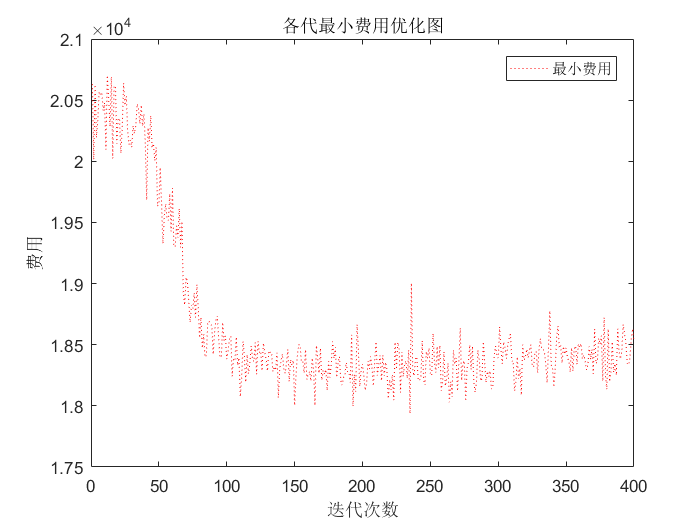
\includegraphics[width=0.8\linewidth]{ch6-2-2.png}
            \caption{}
        \end{minipage}
    \end{subfigure}\\
    \begin{subfigure}[t]{0.5\linewidth}
        \captionsetup{justification=centering}
        \begin{minipage}[b]{1\linewidth}
            \centering
            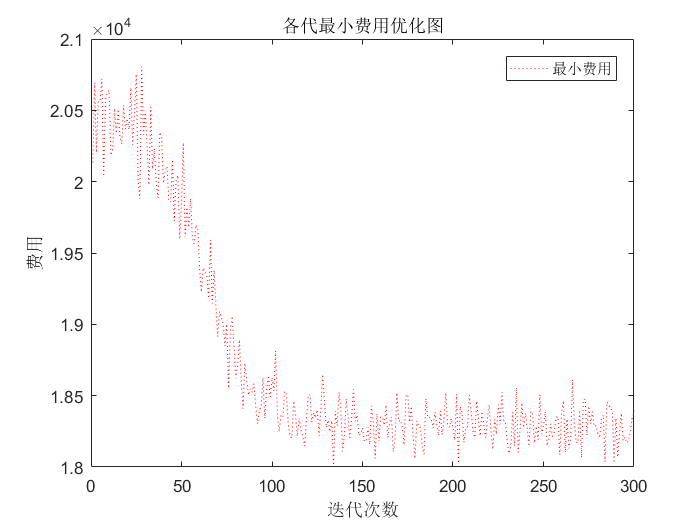
\includegraphics[width=0.8\linewidth]{ch6-2-3.png}
            \caption{}
        \end{minipage}
    \end{subfigure}
    \hspace{-5em}
    \begin{subfigure}[t]{0.5\linewidth}
        \captionsetup{justification=centering}
        \begin{minipage}[b]{1\linewidth}
            \centering
            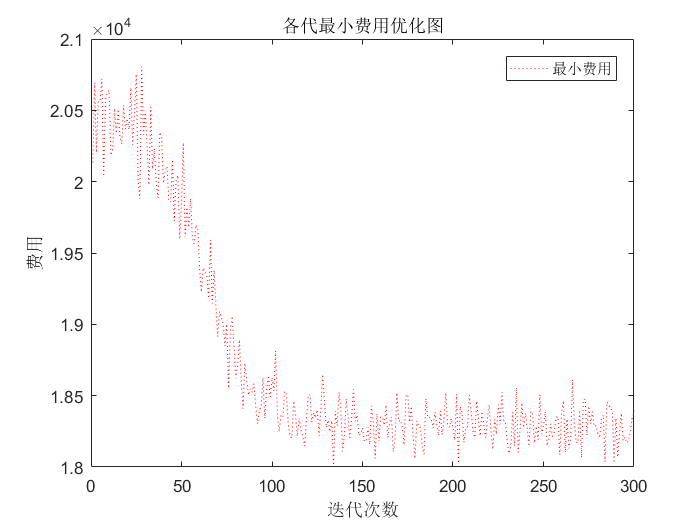
\includegraphics[width=0.8\linewidth]{ch6-2-3.png}
            \caption{}
        \end{minipage}
    \end{subfigure}
    \caption{不同迭代次数对比}
    \label{f.ch6-2}
\end{figure}
%%%%%%%%%%%%%%%%%%%%%%%%%%%%%%%%参考文献插入示例%%%%%%%%%%%%%%%%

% 后置部分
\backmatter

% 结论:在结论相应的 TeX 文件处进行结论部分的撰写
% %%
% The BIThesis Template for Bachelor Graduation Thesis
%
% 上海电力大学毕业设计(论文)中英文摘要 —— 使用 XeLaTeX 编译
%
% Copyright 2020-2023 SUEPaper
%
% This work may be distributed and/or modified under the
% conditions of the LaTeX Project Public License, either version 1.3
% of this license or (at your option) any later version.
% The latest version of this license is in
%   http://www.latex-project.org/lppl.txt
% and version 1.3 or later is part of all distributions of LaTeX
% version 2005/12/01 or later.
%
% This work has the LPPL maintenance status `maintained'.
%
% The Current Maintainer of this work is Haiwen Zhang.
%%

\begin{conclusion}
  % 结论部分尽量不使用 \subsection 二级标题,只使用 \section 一级标题

  % 这里插入一个参考文献,仅作参考
  本文结论……。\cite{李成智2004飞行之梦}

  \textcolor{blue}{结论作为毕业设计(论文)正文的最后部分单独排写,但不加章号。结论是对整个论文主要结果的总结。在结论中应明确指出本研究的创新点,对其应用前景和社会、经济价值等加以预测和评价,并指出今后进一步在本研究方向进行研究工作的展望与设想。结论部分的撰写应简明扼要,突出创新性。阅后删除此段。}

  \textcolor{blue}{结论正文样式与文章正文相同:宋体、小四;行距:1.25 倍行距;间距段前段后均为 0 行。阅后删除此段。}
\end{conclusion}


% 致谢:在致谢相应的 TeX 文件处进行致谢部分的撰写
%%
% The BIThesis Template for Bachelor Graduation Thesis
%
% 上海电力大学毕业设计(论文)中英文摘要 —— 使用 XeLaTeX 编译
%
% Copyright 2020-2023 SUEPaper
%
% This work may be distributed and/or modified under the
% conditions of the LaTeX Project Public License, either version 1.3
% of this license or (at your option) any later version.
% The latest version of this license is in
%   http://www.latex-project.org/lppl.txt
% and version 1.3 or later is part of all distributions of LaTeX
% version 2005/12/01 or later.
%
% This work has the LPPL maintenance status `maintained'.
%
% The Current Maintainer of this work is Haiwen Zhang.
%%

\begin{acknowledgements} 

感谢最先制作出中南大学博士学位论文 LaTeX 模板的郭大侠@CSGrandeur。

感谢添加本科学位论文样式支持的@BlurryLight。

感谢帮助重构项目并进行测试的@burst-bao以及为独立使用LaTeX进行毕业论文写作提供宝贵经验的16级的姜析阅学长。

感谢所有为模板贡献过代码的同学们!

\end{acknowledgements}

% 参考文献:如无特殊需要,参考文献相应的 TeX 文件无需改动,添加参考文献请使用 BibTeX 的格式
%   添加至 misc/ref.bib 中,并在正文的相应位置使用 \cite{xxx} 的格式引用参考文献
%%
% The SUEPThesis Template for Bachelor Graduation Thesis
%
% 上海电力大学毕业设计(论文)中英文摘要 —— 使用 XeLaTeX 编译
%
% Copyright 2020-2023 SUEPaper
%
% This work may be distributed and/or modified under the
% conditions of the LaTeX Project Public License, either version 1.3
% of this license or (at your option) any later version.
% The latest version of this license is in
%   http://www.latex-project.org/lppl.txt
% and version 1.3 or later is part of all distributions of LaTeX
% version 2005/12/01 or later.
%
% This work has the LPPL maintenance status `maintained'.
%
% The Current Maintainer of this work is Haiwen Zhang.
%%

\begin{bibprint}

% -------------------------------- 示例内容(正式使用时请删除) ------------------------------------- %

% 抑制多次调用 \printbibliography 的 warning,只有示例代码会需要此语句。
\BiblatexSplitbibDefernumbersWarningOff

\textcolor{blue}{参考文献书写规范}

\textcolor{blue}{参考国家标准《信息与文献参考文献著录规则》【GB/T 7714—2015】,参考文献书写规范如下:}

\textcolor{blue}{\textbf{1. 文献类型和标识代码}}

\textcolor{blue}{普通图书:M}\qquad\textcolor{blue}{会议录:C}\qquad\textcolor{blue}{汇编:G}\qquad\textcolor{blue}{报纸:N}

\textcolor{blue}{期刊:J}\qquad\textcolor{blue}{学位论文:D}\qquad\textcolor{blue}{报告:R}\qquad\textcolor{blue}{标准:S}

\textcolor{blue}{专利:P}\qquad\textcolor{blue}{数据库:DB}\qquad\textcolor{blue}{计算机程序:CP}\qquad\textcolor{blue}{电子公告:EB}

\textcolor{blue}{档案:A}\qquad\textcolor{blue}{舆图:CM}\qquad\textcolor{blue}{数据集:DS}\qquad\textcolor{blue}{其他:Z}

\textcolor{blue}{\textbf{2. 不同类别文献书写规范要求}}

\textcolor{blue}{\textbf{期刊}}

\noindent\textcolor{blue}{[序号]主要责任者. 文献题名[J]. 刊名, 出版年份, 卷号(期号): 起止页码. }

\printbibliography [type=article,heading=none] 

\textcolor{blue}{\textbf{普通图书}}

\noindent\textcolor{blue}{[序号]主要责任者. 文献题名[M]. 出版地: 出版者, 出版年. 起止页码. }
\cite{Raymer1992Aircraft}

\printbibliography [keyword={book},heading=none] 

\textcolor{blue}{\textbf{会议论文集}}

\noindent\textcolor{blue}{[序号]析出责任者. 析出题名[A]. 见(英文用In): 主编. 论文集名[C]. (供选择项: 会议名, 会址, 开会年)出版地: 出版者, 出版年. 起止页码. }
\cite{sunpinyi}

\printbibliography [type=inproceedings,heading=none] 

\textcolor{blue}{\textbf{专著中析出的文献}}

\noindent\textcolor{blue}{[序号]析出责任者. 析出题名[A]. 见(英文用In): 专著责任者. 书名[M]. 出版地: 出版者, 出版年.起止页码. }
\cite{luoyun}

\printbibliography [type=inbook,heading=none] 

\textcolor{blue}{\textbf{学位论文}}

\noindent\textcolor{blue}{[序号]主要责任者. 文献题名[D]. 保存地: 保存单位, 年份. }
\cite{zhanghesheng}
\cite{Sobieski}

\printbibliography [keyword={thesis},heading=none] 

\textcolor{blue}{\textbf{报告}}

\noindent\textcolor{blue}{[序号]主要责任者. 文献题名[R]. 报告地: 报告会主办单位, 年份. }
\cite{fengxiqiao}
\cite{Sobieszczanski}

\printbibliography [keyword={techreport},heading=none] 

\textcolor{blue}{\textbf{专利文献}}

\noindent\textcolor{blue}{[序号]专利所有者. 专利题名[P]. 专利国别: 专利号, 发布日期. }
\cite{jiangxizhou}

\printbibliography [type=patent,heading=none] 

\textcolor{blue}{\textbf{国际、国家标准}}

\noindent\textcolor{blue}{[序号]标准代号. 标准名称[S]. 出版地: 出版者, 出版年. }
\cite{GB/T16159—1996}

\printbibliography [keyword={standard},heading=none] 

\textcolor{blue}{\textbf{报纸文章}}

\noindent\textcolor{blue}{[序号]主要责任者. 文献题名[N]. 报纸名, 出版年, 月(日): 版次. }
\cite{xiexide}

\printbibliography [keyword={newspaper},heading=none] 

\textcolor{blue}{\textbf{电子文献}}

\noindent\textcolor{blue}{[序号]主要责任者. 电子文献题名[文献类型/载体类型]. 电子文献的出版或可获得地址(电子文献地址用文字表述), 发表或更新日期/引用日期(任选). }
\cite{yaoboyuan}

\printbibliography [keyword={online},heading=none] 

\textcolor{blue}{关于参考文献的未尽事项可参考国家标准《信息与文献参考文献著录规则》(GB/T 7714—2015)}

\textcolor{red}{以下是真正的参考文献}
% -------------------------------- 示例内容(正式使用时请删除) ------------------------------------- %

% 在使用时,请删除/注释上方示例内容,并启用下方语句以输出所有的参考文献
\printbibliography[heading=none]
\end{bibprint}

% 附录:在附录相应的 TeX 文件处进行附录部分的撰写
%%
% The BIThesis Template for Bachelor Graduation Thesis
%
% 上海电力大学毕业设计(论文)中英文摘要 —— 使用 XeLaTeX 编译
%
% Copyright 2020-2023 SUEPaper
%
% This work may be distributed and/or modified under the
% conditions of the LaTeX Project Public License, either version 1.3
% of this license or (at your option) any later version.
% The latest version of this license is in
%   http://www.latex-project.org/lppl.txt
% and version 1.3 or later is part of all distributions of LaTeX
% version 2005/12/01 or later.
%
% This work has the LPPL maintenance status `maintained'.
%
% The Current Maintainer of this work is Haiwen Zhang.
%%

\chapter{附录代码}

附录部分用于存放这里用来存放不适合放置在正文的大篇幅内容、典型如代码、图纸、完整数学证明过程等内容。

\section{堆溢出检测算法}

\begin{algorithm}[h]
    \caption{堆溢出检测算法}\label{alg:ovf}
    \begin{algorithmic}[1]
        \IF {$\beta \in \mathbb{N^{*}} \land \Delta_\beta = \Delta_{\beta - 1} \land \beta < S$}
            \STATE 正常写入
        \ELSIF {$\beta \in \mathbb{N^{*}} \land \Delta_\beta \neq \Delta_{\beta - 1} \land \beta \geq S$}
            \STATE 发生堆溢出
        \ENDIF
    \end{algorithmic}
\end{algorithm}


\chapter{康托尔辩辞录:数学的自由与制约}

(录自康托尔:《一般集合论基础》,1883)

数学在其发展中是完全自由的,它只受下述自明的关注所制约,即它的概念既要内在地不存在矛盾,还要参与确定与此前形成的,已经存在着地和已被证明地概念之关系(借助定义贯串起来)。特别地,在引入新数时,数学只遵循:在给出它们地定义时使之具有某种确定性,并且在某些情况下,使之与老数有某种关系,在特定地场合中这种关系一定会使它们(新数和老数)互相区别开来,只要一个数满足这些条件,数学只能而且必须把它看作是存在的和实在的东西,这正是我……关于为什么必须把有理数、无理数和复数看作与有限正整数一样是实在的所建议的理由。

我相信,没有必要害怕,许多人是害怕,这些原则含有对于科学的危险,一方面,实行造出新数的自由必须服从所设计的条件,但这些条件给任意性留下的活动空间是非常小的。而且,每一数学概念在其自身之中也带有必要的矫正物;如果它没有收获也不合适(它的无用很快就会表明这一点),那么它将由于没有成功而被丢弃。另一方面,在我看来,对于数学研究工作的任何多余的限制只会随之而带来更大的危险,由于实际上并没有任何理由可说明它是由科学的本质推断出来的,它的危险就更大了,而数学的本质恰恰在于它的自由。

如果高斯、柯西、阿贝尔、雅可比、狄利克雷、魏尔斯特拉斯、埃尔米特和黎曼总是被束缚而拿他们的新想法去臣服于形而上学的控制,那么,我们今日就不可能为现代函数论的雄伟建筑而高兴,现代函数论的设计和矗立是完全自由的,毫无短视的瞬间目的……。如果福克斯、庞加莱和其他许多杰出的智者受外来影响所包围和限制,我们就会见不到他们带给微分方程论的巨大的推动,还有,如果枯莫尔不是斗胆地(大有仿效者)把所谓的“理想”数引入数论,我们今天也无从去羡慕钦佩克罗内克和戴德金在代数和算术上十分重要和杰出的工作。

因此,如已说明的,数学是要脱离形而上学的桎梏而完全自由地发展 \dots



% \end{appendixs}



\end{document}
